\documentclass[tikz, preview]{standalone}

\usepackage{amsfonts, amsthm, amssymb, amsmath, stmaryrd, etoolbox}
\usepackage{tikz}
\usetikzlibrary{matrix,arrows}

\begin{document}
\[
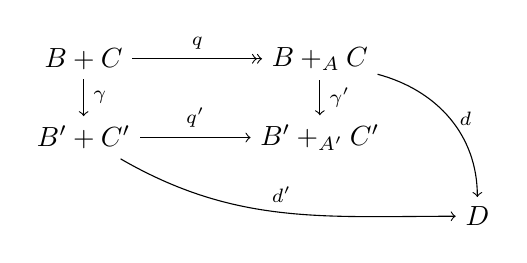
\begin{tikzpicture}[baseline=(current  bounding  box.center)]
\node (BC) at (-1,1) {$B+C$};
\node (BAC) at (2,1) {$B+_AC$};
\node (BC') at (-1,0) {$B'+C'$};
\node (BAC') at (2,0) {$B'+_{A'}C'$};
\node (D) at (4,-1) {$D$};
%
\draw [font=\scriptsize,->>] (BC) edge node[above] {$q$} (BAC);
\draw [font=\scriptsize,->] (BC) edge node[right] {$\gamma$} (BC');
\draw [font=\scriptsize,->] (BAC) edge node[right] {$\gamma'$} (BAC');
\draw [font=\scriptsize,->] (BAC) edge [out=-15,in=90] node[right] {$d$} (D);
\draw [font=\scriptsize,->.] (BC') edge node[above] {$q'$} (BAC');
\draw [font=\scriptsize,->] (BC') edge[out=-30,in=180] node[above] {$d'$} (D);
\end{tikzpicture}
\]
\end{document}
